\documentclass[lecture,12pt,]{pcms-l}
\input preamble.tex

% For faster processing, load Matlab syntax for listings
\definecolor{MyDarkGreen}{rgb}{0.0,0.4,0.0}
\lstloadlanguages{Matlab}%
\lstset{language=Matlab,
        frame=single,
        basicstyle=\small\ttfamily,
        keywordstyle=[1]\color{Blue}\bf,
        keywordstyle=[2]\color{Purple},
        keywordstyle=[3]\color{Blue}\underbar,
        identifierstyle=,
        commentstyle=\usefont{T1}{pcr}{m}{sl}\color{MyDarkGreen}\small,
        stringstyle=\color{Purple},
        showstringspaces=false,
        tabsize=5,
        % Put standard MATLAB functions not included in the default
        % language here
        morekeywords={xlim,ylim,var,alpha,factorial,poissrnd,normpdf,normcdf},
        % Put MATLAB function parameters here
        morekeywords=[2]{on, off, interp},
        % Put user defined functions here
        morekeywords=[3]{FindESS},
        morecomment=[l][\color{Blue}]{...},
        numbers=left,
        firstnumber=1,
        numberstyle=\tiny\color{Blue},
        stepnumber=0
        }

% Only the next five fields need to be edited.
\newcommand{\lecAuth}{R.A. de Callafon}
\newcommand{\scribe}{Thomas Denewiler}
\newcommand{\authEmail}{callafon@ucsd.edu}
\newcommand{\scribeEmail}{tdenewiler@gmail.com}
\newcommand{\course}{MAE 283: Parameter Estimation}
\newcommand{\lectureNum}{7}

\address{Department of Mechanical and Aerospace Engineering, University of California, San Diego}

% Adds a hyperlink to an email address.
\newcommand{\mailto}[2]{\href{mailto:#1}{#2}}

% These commands set the document properties for the PDF output. Needs the hyperref package.
\hypersetup
{
    colorlinks,
    linkcolor={black},
    citecolor={black},
    filecolor={black},
    urlcolor={black},
    pdfauthor={\scribe <\mailto{\scribeEmail}{\scribeEmail}>},
    pdfsubject={\course},
    pdftitle={Lecture \lectureNum},
    pdfkeywords={UC San Diego, Parameter Estimation, System Identification},
    pdfstartpage={1},
}

% Includes a figure
% The first parameter is the label, which is also the name of the figure
%   with or without the extension (e.g., .eps, .fig, .png, .gif, etc.)
%   IF NO EXTENSION IS GIVEN, LaTeX will look for the most appropriate one.
%   This means that if a DVI (or PS) is being produced, it will look for
%   an eps. If a PDF is being produced, it will look for nearly anything
%   else (gif, jpg, png, et cetera). Because of this, when I generate figures
%   I typically generate an eps and a png to allow me the most flexibility
%   when rendering my document.
% The second parameter is the width of the figure normalized to column width
%   (e.g. 0.5 for half a column, 0.75 for 75% of the column)
% The third parameter is the caption.
\newcommand{\scalefig}[3]{
  \begin{figure}[ht!]
    % Requires \usepackage{graphicx}
    \centering
	\fbox{
	    \includegraphics[width=#2\columnwidth]{#1}
	}
    %%% I think \captionwidth (see above) can go away as long as
    %%% \centering is above
    %\captionwidth{#2\columnwidth}%
    \caption{#3}
    \label{#1}
  \end{figure}}

% Includes a MATLAB script.
% The first parameter is the label, which also is the name of the script
%   without the .m.
% The second parameter is the optional caption.
\newcommand{\matlabscript}[2]
  {\begin{itemize}\item[]\lstinputlisting[caption=#2,label=#1]{#1.m}\end{itemize}}

% Example environment.
\newtheoremstyle{example}{\topsep}{\topsep}	%
     {}%         Body font
     {}%         Indent amount (empty = no indent, \parindent = para indent)
     {\bfseries}% Thm head font
     {}%        Punctuation after thm head
     {\newline}%     Space after thm head (\newline = linebreak)
     {\thmname{#1}\thmnumber{ #2}\thmnote{ #3}}%         Thm head spec

   \theoremstyle{example}
   \newtheorem{example}{Example}[section]

% A command to show a vector norm that will have the pipe signs scale with the contents.
\newcommand{\vectornorm}[1]{\left|\left|#1\right|\right|}

% Commands for time and frequency integrals over infinty, cos and sin.
\newcommand{\tint}{\int_{t=-\infty}^\infty}
\newcommand{\fint}{\int_{\omega=-\infty}^\infty}
\newcommand{\tauint}{\int_{\tau=0}^\infty}
\newcommand{\w}{\omega}
\newcommand{\wo}{\omega_0}
\newcommand{\ejwt}{e^{j\omega t}}
\newcommand{\emjwt}{e^{-j\omega t}}
\newcommand{\dt}{\Delta T}


%%%%%%%%%%%%%%%%%%%%%%%%%%%%%%%%%%%%%%%%%%%%%%%%%%%%%%%%%%%%%


\begin{document}
\mainmatter
\setcounter{page}{1}

\lectureseries[\course]{\course}

\auth[R.A. de Callafon]{Lecturer: \lecAuth\\ Scribe: \scribe}
\date{October 15, 2009}

\setaddress

% the following hack starts the lecture numbering at 7
\setcounter{lecture}{6}
\setcounter{chapter}{6}

\lecture{Spectral Analysis and Least Squares}

\section{Spectral Analysis Review}
Figure \ref{fig:07overview} shows an overview of parameter estimation. Up to this point we have worked on estimating the impulse response and the frequency response, which corresponds to Chapters 1,2, and 6 in the Ljung textbook.

\begin{figure}[ht!]
  \centering
  \includegraphics[width=1\textwidth]{images/07overview}
  \caption{Overview of parameter estimation.}
  \label{fig:07overview}
\end{figure}

\begin{figure}[ht!]
  \centering
  \subfloat[Free-body diagram of mass spring damper system.]{
    \label{fig:07fbd}\includegraphics[width=0.4\textwidth]{images/07fbd}
  } \hfill
  \subfloat[Frequency response with variance.]{
    \label{fig:07freqResp}\includegraphics[width=0.4\textwidth]{images/07freqResp}
  } \hfill
  \caption{Frequency response of a mass spring damper system.}
  \label{fig:07msd}
\end{figure}

\begin{figure}[ht!]
  \centering
  \subfloat[Large variance, small bias.]{
    \label{fig:07largeSigma}\includegraphics[width=0.4\textwidth]{images/07largeSigma}
  } \hfill
  \subfloat[Small variance, large bias.]{
    \label{fig:07smallSigma}\includegraphics[width=0.4\textwidth]{images/07smallSigma}
  } \hfill
  \caption{Trade-off between variance and bias when averaging the spectrum.}
  \label{fig:07tradeoff}
\end{figure}

\begin{figure}[ht!]
  \centering
  \includegraphics[width=.5\textwidth]{images/07spectrum}
  \caption{Spectrum of the noise, $v(t)$.}
  \label{fig:07spectrum}
\end{figure}

\begin{figure}[ht!]
  \centering
  \subfloat[Magnitude of the spectrum.]{
    \label{fig:07mag}\includegraphics[width=0.4\textwidth]{images/07mag}
  } \hfill
  \subfloat[Phase of the spectrum.]{
    \label{fig:07phase}\includegraphics[width=0.4\textwidth]{images/07phase}
  } \hfill
  \caption{Magnitude and phase of the spectrum.}
  \label{fig:07magphase}
\end{figure}

\begin{figure}[ht!]
  \centering
  \includegraphics[width=.4x\textwidth]{images/07ls}
  \caption{Least squares projection.}
  \label{fig:07ls}
\end{figure}


\end{document}

%%%%%%%%%%%%%%%%%%%%%%%%%%%%%%%%%%%%%%%%%%%%%%%%%%%%%%%%%%%%%